\documentclass[12pt]{article}
\usepackage{amsmath}
\usepackage{amssymb}
\usepackage{amsthm}
\usepackage{graphicx}
\begin{document}

\begin{flushleft}
Scott Clark \\
MPIPKS
\end{flushleft}

\section{Introduction}

We want to examine the extreme statistics of "Gaussian seas" which are superpositions of plane waves with normally distributed amplitudes. We will look at both the real and complex case and numerically determine the density of maxima and the distribution of the values of the maxima for these two cases as well as other statistically significant information.

\subsection{Real Case}

The function that we are examining in the real case is

\[f(x,y) = \sum_{i = 1}^{N} a_{i} \sin \left(\frac{\sin(\theta_{i}) x}{\lambda/2 \pi} + \frac{cos(\theta_{i}) y}{\lambda/2 \pi} + \delta_{i} \right)\]

where each $a_{i}$ independent and identically normally distributed with mean 0 and variance 1 (N(0,1)). And each $\theta_{i}, \delta_{i}$ is independent and identically uniformly distributed from 0 to $2\pi$.

\subsection{Complex Case}

The function that we are examining in the complex case is

\[\Psi(x,y) = \sum_{i = 1}^{N} a_{i} \cos \left(\frac{\sin(\theta_{i}^{(1)}) x}{\lambda/2 \pi} + \frac{cos(\theta_{i}^{(1)}) y}{\lambda/2 \pi} + \delta_{i}^{(1)} \right) + b_{i} i \sin \left(\frac{\sin(\theta_{i}^{(2)}) x}{\lambda/2 \pi} + \frac{cos(\theta_{i}^{(2)}) y}{\lambda/2 \pi} + \delta_{i}^{(2)} \right)\]
where each $a_{i}$ and $b_{i}$ is independent and identically normally distributed with mean 0 and variance 1 (N(0,1)). And each $\theta_{i}^{(1)}, \theta_{i}^{(2)}, \delta_{i}^{(1)}, \delta_{i}^{(2)}$ is independent and identically uniformly distributed from 0 to $2\pi$.

\section{Density of maxima}

\subsection{Real Case}

\subsubsection{Scaling with area}

To test dependence we superimposed 1000 plane waves of varying amplitudes and heights and found how many local maximums (of $\Psi^{2}$) we could find in different areas ($A = 100, 400, 900, \ldots, 100^{2}$) with the wavelength $\lambda$ set to $2 \pi$. The test was run for 100 different sets of 1000 waves to create some statistical stability. The results are as follows,

\begin{figure}[ht]
	\centering
		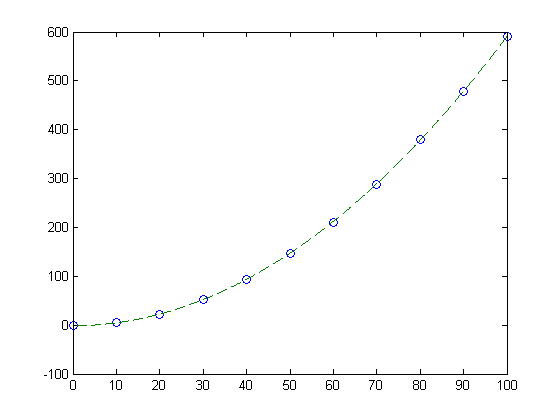
\includegraphics[width=1.00\textwidth]{ascaleSquares.png}
	\caption{Local maximums found of $\Psi^{2}$ versus L, the length of a side of the square area examined.}
	\label{fig:ascaleSquares}
\end{figure}

\pagebreak

As we can see the relation looks to be one of $n \propto L^{2}$

\subsubsection{Scaling with wavelength}

Now we want to test the wavelength ($\lambda$) dependence and so we set A = 400 (L = 20) and test the number of nodes observed for $\lambda = 2 \pi, \frac{2 \pi}{2}, \frac{2 \pi}{3}, \ldots, \frac{2 \pi}{10}$. The results are as follows,

\begin{figure}[ht]
	\centering
		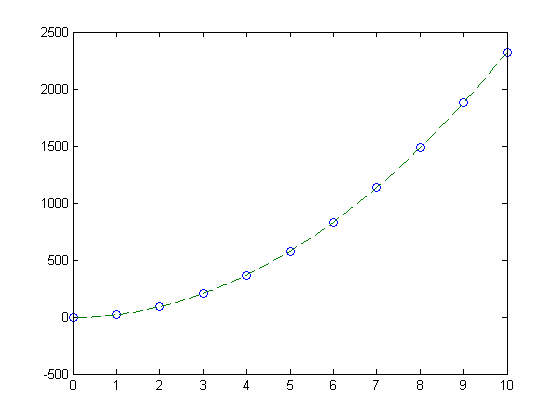
\includegraphics[width=1.00\textwidth]{wlscaleSquares.png}
	\caption{Local maximums found of $\Psi^{2}$ versus z, where $\lambda = \frac{2 \pi}{z}$.}
	\label{fig:wlscaleSquares}
\end{figure}

\pagebreak

Once again we see a quadratic proportionality, $n \propto z^{2} = \frac{1}{\lambda^{2}}$

\subsubsection{Scaling with both parameters}

We put these two realizations together to conclude that the number of local maximums ($n$) of $\Psi^{2}$ observed for any given wavelength in a box of size A is approximately governed by the function,

\[n_{max} \propto \frac{A}{\lambda^{2}}\]

For the exact constant we turn to the previously derived analytics~\cite{LH21} and conclude

\[n_{max,f} = \frac{\pi}{2 \sqrt{3}} \frac{A}{\lambda^{2}} = 0.9070 \frac{A}{\lambda^{2}}\]

what we are concerned with is $\Psi^{2}$ which will have a coefficient of exactly twice this because all minima will become maxima and the quadratic function is monotonic so all maxima will be preserved. So we have

\[n_{max,f^{2}} = \frac{\pi}{\sqrt{3}} \frac{A}{\lambda^{2}} = 1.8138 \frac{A}{\lambda^{2}}\]

and we test this against the number of average number of maxima found for a box of length 512, 128 and 1000 waves of wavelength $2\pi$ over 1000 realizations.

\[\frac{(11903.937)(2\pi)^{2}}{512^{2}} = 1.7927\]
\[\frac{(745.831)(2\pi)^{2}}{128^{2}} = 1.79713\]

both of these results are within about 1 percent of the analytic results. They are slightly lower because we use a finite mesh size to discretized space when we are looking for the maxima and this can cause two maxima to become aliased and only count for one on rare occasions.

\subsection{Complex Case}

For the complex case we find the same proportionality dependence between the number of maxima and the area and wavelength,

\[n_{max,|\Psi|^{2}} \propto \frac{A}{\lambda^{2}}\]

and we turn to the previous numeric~\cite{AW75} (approximated from graph) and analytic~\cite{RA98} (weak argument) results to conclude

\[n_{max,|\Psi|^{2}} \approx 2 \frac{A}{\lambda^{2}}\]

this agrees nicely with our numerics for the number of average number of maxima found for a box of length 512, 256 and 1000 waves of wavelength $2\pi$ over 1000 realizations.

\[\frac{(13368.45)(2\pi)^{2}}{512^{2}} = 2.01326\]
\[\frac{(3515.369)(2\pi)^{2}}{256^{2}} = 2.11763\]

\subsection{Result}

These values give us an effective dimensionality of the system. Each maximum represents a node that can be used in a discrete basis for the superposition. We have the two formula for this dimensionality,

\[n_{real} \approx \frac{\pi}{\sqrt{3}} \frac{A}{\lambda^{2}}\]
\[n_{complex} \approx 2 \frac{A}{\lambda^{2}}\]

\section{Mean value of extremes and their standard deviation}

These values will be essential to transforming the distributions of the extremes. We now attempt to numerically derive formulas for the means and standard deviations of extreme points as they correspond to area and wavelength. Below are tables representing key statistical values.

\begin{table}[hpt]
\centering
\begin{tabular}{|c|c|c|c|}
 & Real & & \\
 \hline
 L & $\bar{\#}_{max}$ & $\bar{x}_{ex}$ & $\sigma_{ex}$ \\
 \hline
 8 & 2.299 & 3942 & 1433.8\\
 16 & 10.429 & 5127 & 1487.4\\
 32 & 44.488 & 6933 & 1565.1\\
 64 & 183.473 & 8217 & 1642.4\\
 128 & 745.831 & 9568 & 1599.6\\
 256 & 1850.677 & 11324 & 1528.5\\
 512$^{*}$ & 11903.937 & 10833 & -\\
\hline
\end{tabular}
\caption{box length, avg. number of maxima, avg height of extreme values, standard deviation of extreme values. Grid spacing was 0.5 except for those marked with $^{*}$, in which case it was 1.0}
\end{table}

\begin{table}[hpt]
\centering
\begin{tabular}{|c|c|c|c|}
 & Complex & & \\
 \hline
 L & $\bar{\#}_{max}$ & $\bar{x}_{ex}$ & $\sigma_{ex}$ \\
 \hline
 8 & 2.673 & 4194.6 & (1572.3)\\
 16 & 12.199 & 5569.1 & (1623.1)\\
 32 & 52.072 & 7159.5 & 1759.5\\
 64 & 214.751 & 8722.9 & 1634.3\\
 128 & 871.744 & 10263 & 1564.1\\
 256 & 3515.369 & 11807 & 1487.2\\
 512$^{*}$ & 13368.45 & 12778 & 1395.2\\
\hline
\end{tabular}
\caption{box length, avg. number of maxima, avg height of extreme values, standard deviation of extreme values. Grid spacing was 0.5 except for those marked with $^{*}$, in which case it was 1.0}
\end{table}

\subsection{Real Case}

Using a modified least squares (where later points are treated with more emphasis) we are able to obtain a function for the mean value of the highest value of a given superposition (the extreme point) (1000 waves, $\lambda = 2\pi$, box length L, 1000 iterations).

\[\bar{x} \approx 2142.943 \log(0.38265 L)\]

Which can be graphically compared to the data as follows,

\begin{figure}[ht]
	\centering
		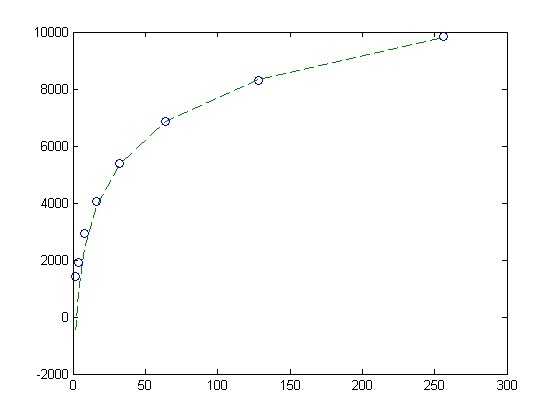
\includegraphics[width=1.00\textwidth]{avgExVsAreal.png}
	\caption{mean extreme val vs L real}
	\label{fig:avgExVsAreal}
\end{figure}

We can derive a formula similar to this using known values of the system namely the maxima density and the mean value of the field.

\[\bar{x} \approx 2 \bar{x}_{field} \log(\pi \#_{max}) \approx 1000 \log(\pi \frac{\pi}{\sqrt{3}} \frac{A}{\lambda^{2}})\]

The standard deviation looks to be nearly constant, although like the complex case it may have a negative logarithmic dependence on box length.

\[\sigma \approx 1584\]

\subsection{Complex Case}

Using a modified least squares (where later points are treated with more emphasis) we are able to obtain a function for the mean value of the highest value of a given superposition (1000 waves, $\lambda = 2\pi$, box length L, 1000 iterations).

\[\bar{x} \approx 2191.779 \log(0.8384 L)\]

Which can be graphically compared to the data as follows,

\begin{figure}[hpt]
	\centering
		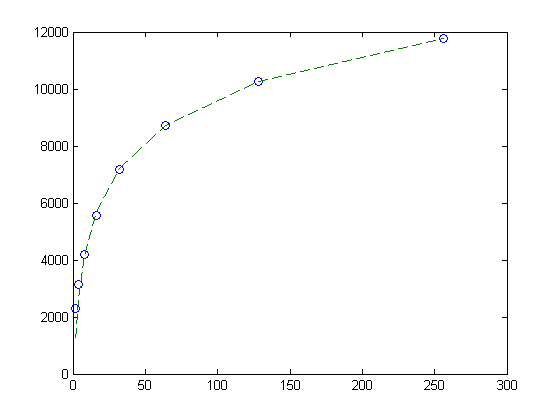
\includegraphics[width=1.00\textwidth]{avgExVsAcomp.png}
	\caption{mean ex val vs L complex}
	\label{fig:avgExVsAcomp}
\end{figure}

This can also be seen to fit more closely to the analytic results of~\cite{RA98} which state that the largest maximum should scale like

\[\bar{x} = |\psi|_{\infty} \propto c\sqrt{\log{E_{n}}}\]

Using a least squares fitting we obtain the results in the plot below which far outperforms the other model of

\[\bar{x} \approx 2 \bar{x}_{max} \log{\#_{max}}\]

as seen by the plot below,

\begin{figure}[hpt]
	\centering
		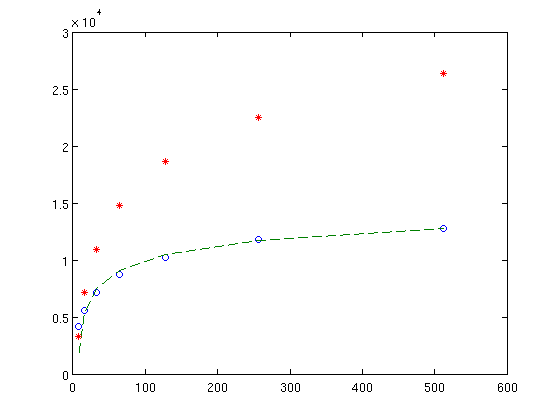
\includegraphics[width=1.00\textwidth]{complex_meanEx_wLog.png}
	\caption{Mean value of extremes using the 2 theoretical models, dashed from~\cite{RA98}}
	\label{fig:complex_meanEx_wLog}
\end{figure}


Using a modified least squares (where later points are treated with more emphasis) we are able to obtain a function for the standard deviation of the highest value of a given superposition (1000 waves, $\lambda = 2\pi$, box length L, 1000 iterations).

\[\sigma \approx 2187.859 + 127.975\log(\frac{1}{L}) \ \ \ L \geq 32\]

\[\sigma \approx 127.975\log(\frac{2.65885E7}{L}) \ \ \ L \geq 32\]

Which was used as a prediction for the $\sigma$ of $L=512$ with the following results,

\[\sigma_{pred} = 1395.59\]
and
\[\sigma_{num} = 1395.2\]
so we can see that the standard deviation does drop like $\log(\frac{1}{L})$ which is what we would expect if
\[e^{1/b} \propto L^{2}\]

\begin{figure}[hpt]
	\centering
		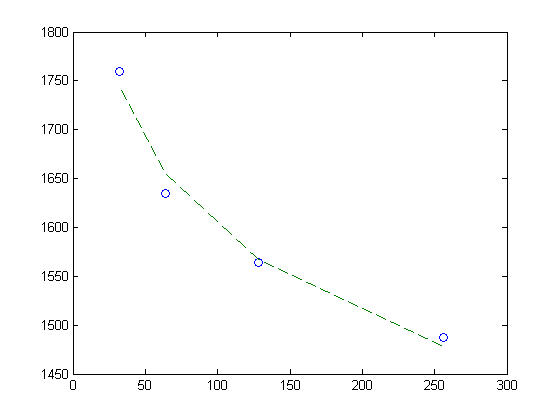
\includegraphics[width=1.00\textwidth]{bcomplex-log.png}
	\caption{Standard deviation vs. box length for $L \geq 32$}
	\label{fig:bcomplex-log}
\end{figure}


\subsection{Mean value of all maxima vs. mean value of field}

\subsubsection{Real Case}

The average mean value of a maximum in the system was found to be about 3.66 larger than the average value for the system in general (518.4105). This was done by taking 1000 waves of wavelength $2 \pi$ and superimposing them on a grids from 8x8 to 512x512 with 1000 realizations and taking the average of the maximum heights and the average of every point in the field for each realization and comparing the ratio of the average of these quantities.

\subsubsection{Complex Case}

We can also find the average mean value of each extreme in the system which was found to be 2.779 times larger than the average of the field itself (1000). The test performed was identical to the one above.

\section{Extreme Value Distribution}

With the values calculated above we are now prepared to examine how the extreme values (greatest valued point) of our planar superpositions vary.

\subsection{Real Case}

\subsubsection{Fitting to Gumbel by definition}
We must transform the variable (32x32, 2pi, 1000 waves, 40,000 it);
\[Y = \frac{X - a}{b}\]
using the definition
\[b = \frac{\sqrt{6}}{\pi} \sigma = 1253.0\]
\[a = \bar{x} - \gamma b = 4707.1\]

\begin{figure}[hpt]
	\centering
		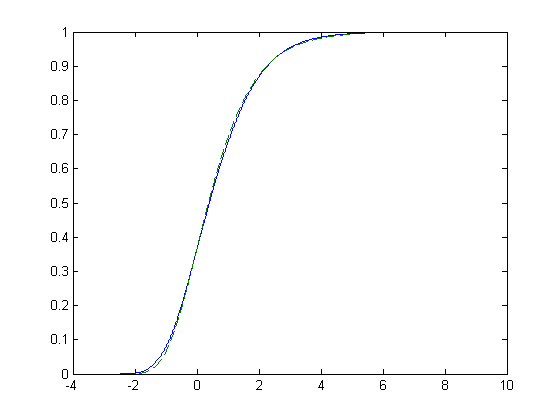
\includegraphics[width=1.00\textwidth]{40000it32x32gumbR.png}
	\caption{Distribution of extreme points as transformed by definition (real, 40000 iterations)}
	\label{fig:40000it32x32gumbR}
\end{figure}

\subsubsection{Predictive fitting}
from above we know
\[\bar{x} \approx 2142.943 log(0.38265*L)\]
and
\[\sigma \approx 1584.0\]
from this we can obtain the linear transformation
\[b = \frac{\sqrt{6}}{\pi}1584.0 = 1235.0\]
\[a = 2142.943 log(0.38265*32) - 0.57721\frac{\sqrt{6}}{\pi}1584.0 = 4655.4\]
which looks like

\begin{figure}[hpt]
	\centering
		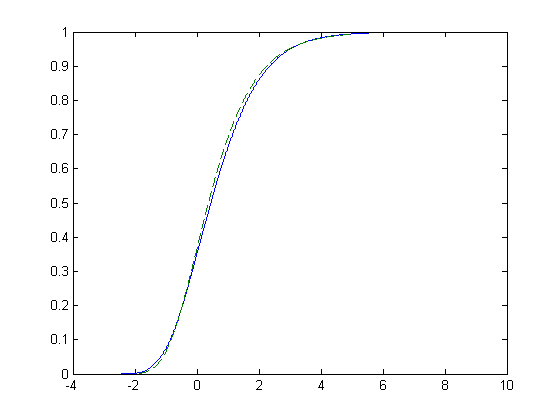
\includegraphics[width=1.00\textwidth]{40000it32x32gumbRpredictive.png}
	\caption{Distribution of extreme points as transformed by prediction (real, 40000 iterations)}
	\label{fig:40000it32x32gumbRpredictive}
\end{figure}

\subsubsection{Distribution of 10 largest maxima for each realization}

We want to find the distribution of the 10 highest maxima of all of the realizations now, not just the very highest one. We immediately notice that this distribution is Gumbel with constants (by definition)

(This is done with 1000 waves of wavelength $2\pi$ on a grid of 512x512 and 1000 realizations, the following 3 sections will have an identical setup)

\[a = 8476.5\]
and
\[b = 942.3357\]

which is a perfect fit,

\begin{figure}[hpt]
	\centering
		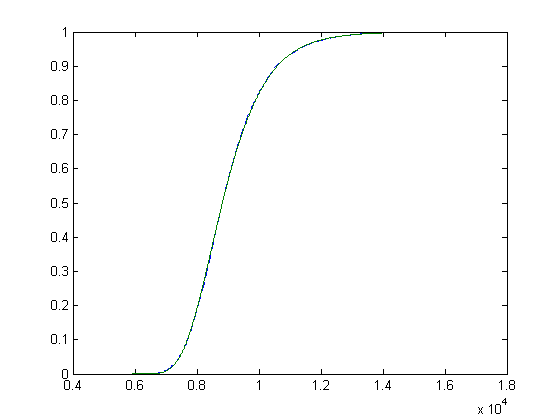
\includegraphics[width=1.00\textwidth]{pnR_512_top10_gumbel.png}
	\caption{1}
	\label{fig:pnR_512_top10_gumbel}
\end{figure}


\subsubsection{Distribution of 10 smallest maxima for each realization}

Now we want to find the distribution of the 10 smallest maxima of each of the distributions. We anticipate that the distribution should be Weibull which has a distribution function as follows,

\[F(x,k,\lambda) = 1 - e^{-(x/\lambda)^{k}}\]

We use a least squares minimization to find the constants

\[\lambda = 65.5\]

\[k = 4\]

which comes to the following results,

\begin{figure}[hpt]
	\centering
		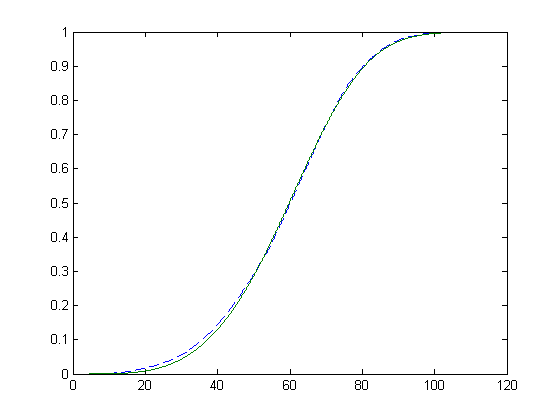
\includegraphics[width=1.00\textwidth]{pnR_512_bot10_weibul.png}
	\caption{2}
	\label{fig:pnR_512_bot10_weibul}
\end{figure}

\subsubsection{Distribution of the difference between the extreme value and 9 next highest maxima}

Now we want to look at the distribution of the distance between the value of the highest point of each realization and the closest 9 maxima. We see that this resembles a Gumbel distribution with constants (by definition)

\[a = 1465.0\]

\[b = 951.8022\]

we see that this is a good fit,

\begin{figure}[hpt]
	\centering
		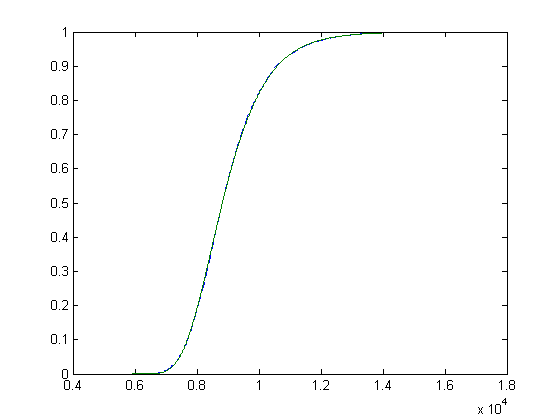
\includegraphics[width=1.00\textwidth]{pnR_512_top10_gumbel.png}
	\caption{3}
	\label{fig:pnR_512_top10_gumbel}
\end{figure}

\subsubsection{Distribution of the difference between the smallest maxima and the 9 next smallest maxima}

Now we want to find the same thing but in the opposite order. We want to find the distribution of the distance between the value of the lowest maxima and the 9 closest maxima to it. This is not immediately obvious what distribution it should be. The following plot is the Gumbel and the Weibul with constants found by definition and least squares respectively.

\begin{figure}[hpt]
	\centering
		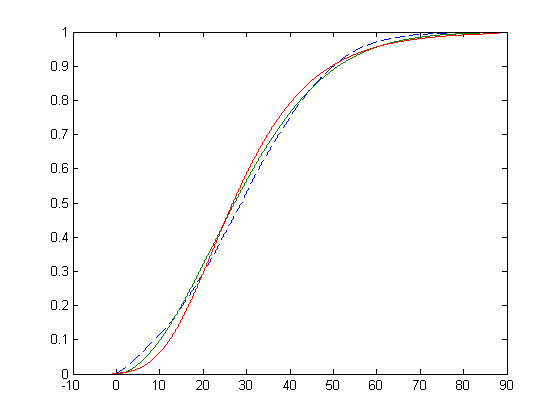
\includegraphics[width=1.00\textwidth]{pnR_512_bot10diff_gumbel_weibull.png}
	\caption{4}
	\label{fig:pnR_512_bot10diff_gumbel_weibull}
\end{figure}

We see that these two distributions seem to fail at representing the value we are interested in. The normal distribution with parameters $\mu = 29.38.78$ and $\sigma = 15.5360$ seems to fit pretty well though,

\begin{figure}[hpt]
	\centering
		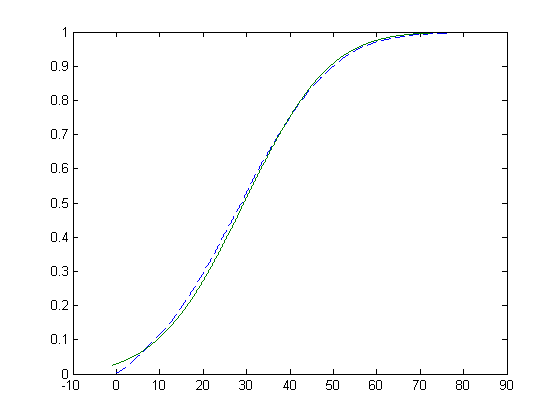
\includegraphics[width=1.00\textwidth]{pnR_512_bot10diff_normal.png}
	\caption{5}
	\label{fig:pnR_512_bot10diff_normal}
\end{figure}

\subsection{Complex Case}

\subsubsection{Fitting to Gumbel by definition}
We want to find if the distribution of the extreme values for different realizations of this superposition fit that of the Gumbel distribution. To do this we superimpose 1000 plane waves of wavelength $2 \pi$ in a 100x100 grid (with discretization width .5) 1000 times and record the largest value for $|\psi|^{2}$ for each. We then make the distribution of these extremes. The idea is that by linearly transforming our random variable by

\[Y = \frac{X - a}{b}\]

We now use a transformation where we fix a and b by the equations
\[\bar{x} = a + \gamma b\]
\[\sigma = \frac{\pi}{\sqrt{6}} b\]
instead of the least squares data fitting. We have
\[\bar{x} = 9639.3\]
\[\sigma = 1610.5\]
which gives us
\[a = 8914.5\]
\[b = 1255.7\]
for the 100x100 case and for the 500x500 case we obtain,
\[\bar{x} = 12684\]
\[\sigma = 1404.7\]
which gives us
\[a = 12051\]
\[b = 1095.3\]
now we look at the distribution compared to that of the Gumbel,

We see that this is a good fit, and even when the area is increased to a box of 500 x 500, the distribution does not change (it is stationary at this point),

\begin{figure}[hpt]
	\centering
		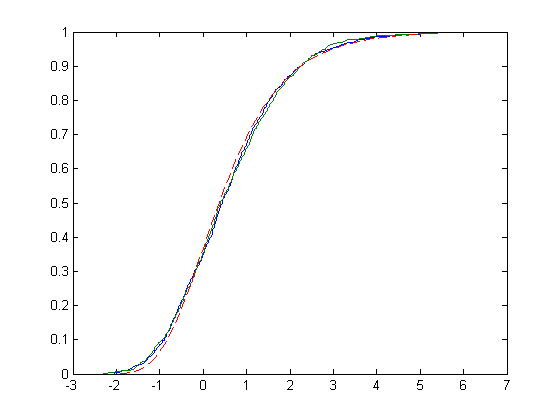
\includegraphics[width=1.00\textwidth]{extremeDistVsGumb.png}
	\caption{Transformed extreme distribution for 100x100 area (blue) vs. transformed extreme distribution for 500x500 area (green) vs. Gumbel (red, dashed)}
	\label{fig:extremeDistVsGumb}
\end{figure}

\pagebreak

\subsubsection{Fitting from definition and large iterations}

now we compute the extreme distribution for many more iterations in a 64x64 area. We preform 25000 iterations. With the following similar results,

\begin{figure}[hpt]
	\centering
		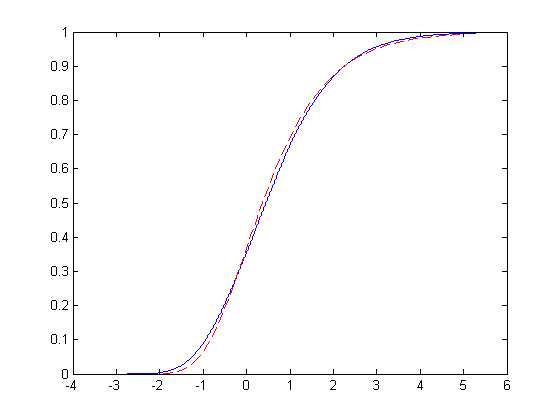
\includegraphics[width=1.00\textwidth]{25000it128x128gumb.png}
	\caption{Transformed distribution of extremes vs. Gumbel distribution (25000 iterations)}
	\label{fig:25000it128x128gumb}
\end{figure}

We can see that the fit improves a little and the resolution becomes much better.

\[a = 7728\]
\[b = 1285.5\]

\subsubsection{Predictive fitting}

Now we use the same definition, only this time we use the predictive fitting from the numerical equations derived in section 3,

\[\bar{x} \approx 2191.779 \log(0.8384 L)\]

\[\sigma \approx 2187.859 - 127.975\log(L) \ \ \ L \geq 32\]

which gives

\[a \approx 2191.779 \log(0.8384 L) - \frac{\gamma \sqrt{6}}{\pi}(2187.859 - 127.975\log(L))\]
\[= -1370.9 + 1124.7 \log(A)\]

\[b \approx \frac{\sqrt{6}}{\pi}(2187.859 - 127.975\log(L)) = 1705.9 - 49.89 \log(A)\]

This gives a very accurate prediction of the gumbel distribution that the extremes fit (256x256, 1000 waves, $\lambda = 2\pi$, 1000 iterations), $a = 11100, b = 1156.8$.

\begin{figure}[hpt]
	\centering
		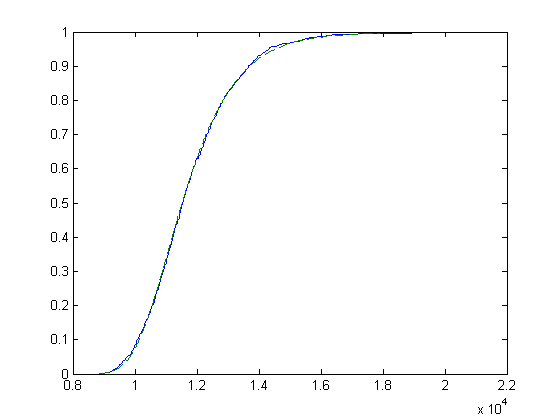
\includegraphics[width=1.00\textwidth]{predictive_gumb_complex.png}
	\caption{Predictive gumbel fit (complex)}
	\label{fig:predictive_gumb_complex}
\end{figure}


\subsubsection{Distribution of 10 largest maxima for each realization}

We want to find the distribution of the 10 highest maxima of all of the realizations now, not just the very highest one. We immediately notice that this distribution is Gumbel with constants (by definition)

(This is done with 1000 waves of wavelength $2\pi$ on a grid of 512x512 and 1000 realizations, the following 3 sections will have an identical setup)

\[a = 10310\]
and
\[b = 937.588\]

which is a perfect fit,

\begin{figure}[hpt]
	\centering
		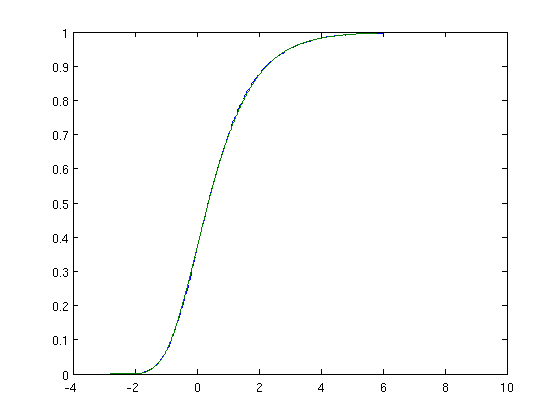
\includegraphics[width=1.00\textwidth]{pnC_512_top10_gumbel.png}
	\caption{1}
	\label{fig:pnC_512_top10_gumbel}
\end{figure}


\subsubsection{Distribution of 10 smallest maxima for each realization}

Now we want to find the distribution of the 10 smallest maxima of each of the distributions. We anticipate that the distribution should be Weibull which has a distribution function as follows,

\[F(x,k,\lambda) = 1 - e^{-(x/\lambda)^{k}}\]

We use a least squares minimization to find the constants

\[\lambda = 273.992\]

\[k = 5.9129\]

which comes to the following results,

\begin{figure}[hpt]
	\centering
		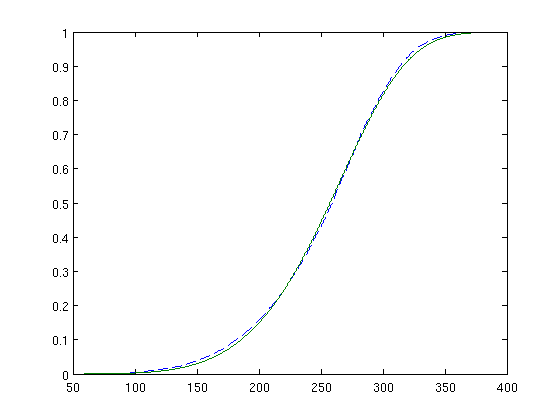
\includegraphics[width=1.00\textwidth]{pnC_512_bot10_weibul.png}
	\caption{2}
	\label{fig:pnC_512_bot10_weibul}
\end{figure}

\subsubsection{Distribution of the difference between the extreme value and 9 next highest maxima}

Now we want to look at the distribution of the distance between the value of the highest point of each realization and the closest 9 maxima. We see that this resembles a Gumbel distribution with constants (by definition)

\[a = 1567.4\]

\[b = 992.6887\]

we see that this is a good fit,

\begin{figure}[hpt]
	\centering
		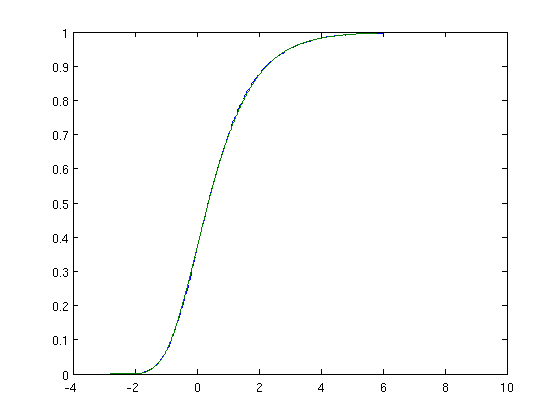
\includegraphics[width=1.00\textwidth]{pnC_512_top10_gumbel.png}
	\caption{3}
	\label{fig:pnC_512_top10_gumbel}
\end{figure}

\subsubsection{Distribution of the difference between the smallest maxima and the 9 next smallest maxima}

Now we want to find the same thing but in the opposite order. We want to find the distribution of the distance between the value of the lowest maxima and the 9 closest maxima to it. This is not immediately obvious what distribution it should be. The following plot is the Gumbel and the Weibul with constants found by definition and least squares respectively.

\begin{figure}[hpt]
	\centering
		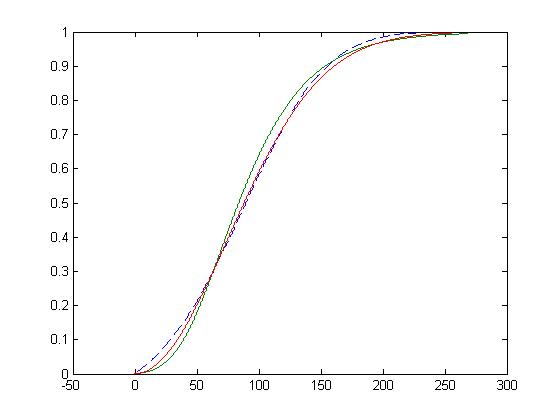
\includegraphics[width=1.00\textwidth]{pnC_512_bot10diff_gumbel_weibull.png}
	\caption{4}
	\label{fig:pnC_512_bot10diff_gumbel_weibull}
\end{figure}

We see that these two distributions seem to fail at representing the value we are interested in. The normal distribution with parameters $\mu = 91.4217$ and $\sigma = 47.6459$ seems to fit pretty well though,

\begin{figure}[hpt]
	\centering
		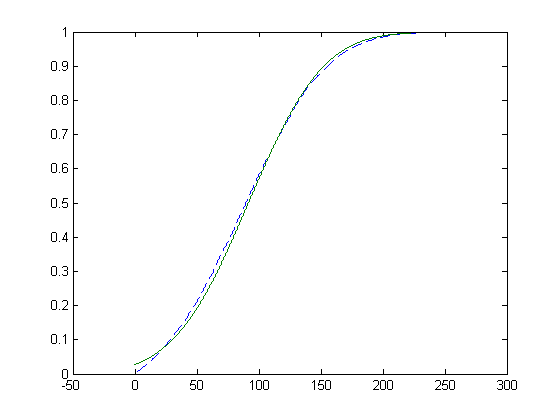
\includegraphics[width=1.00\textwidth]{pnC_512_bot10diff_normal.png}
	\caption{5}
	\label{fig:pnC_512_bot10diff_normal}
\end{figure}
\section{Randomness Tests}

\subsection{Real}

\subsubsection{Point wise correlation}

To ensure that we indeed have a random "gaussian sea" we implement 2 "randomness" tests. The first test takes 1000 random points from a $\Psi$ function that was generated with 1000 plane waves in a 50x50 grid with wavelength $2 \pi$. It then plots the distribution of these points, the idea being that one would want this value to be normally distributed by the central limit theorem. We do just this with the following results,

\begin{figure}[hpt]
	\centering
		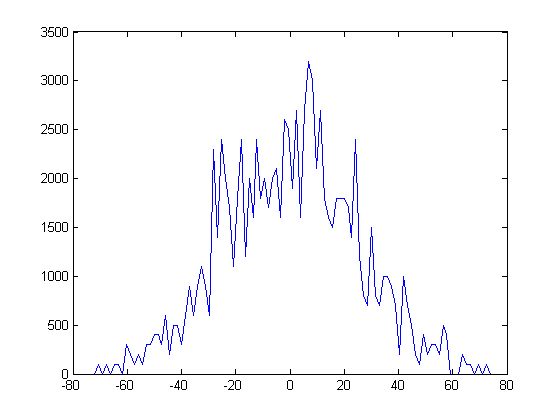
\includegraphics[width=1.00\textwidth]{randomdist1000p50by50wav1000.png}
	\caption{Distribution of 1000 values of random points of a sample $\Psi$.}
	\label{fig:randomdist1000p50by50wav1000}
\end{figure}

\pagebreak

\subsubsection{Autocorrelation matrix}

The next tests involves preforming an autocorrelation of the function ($\Psi$) with itself. The autocorrelation function for 2 dimensional arrays (like our 2D function is) is defined by the matrix,
\[\rho_{ij} = \sum_{m=0}^{M} \sum_{n=0}^{N} \Psi(x_{m},y_{n}) \Psi(x_{m+i (mod M)},y_{n+j (mod N)})\]
What we expect to see is a radially symmetric $J_{0}$ Bessel function which would imply no correlation. In a surface plot of our correlation matrix this would look like a peak at the center rippling out into smaller "waves" to be eventually met by 8 other peaks which are artifacts of the modulus in the definition. The results we obtained are as follows,

\begin{figure}[hpt]
	\centering
		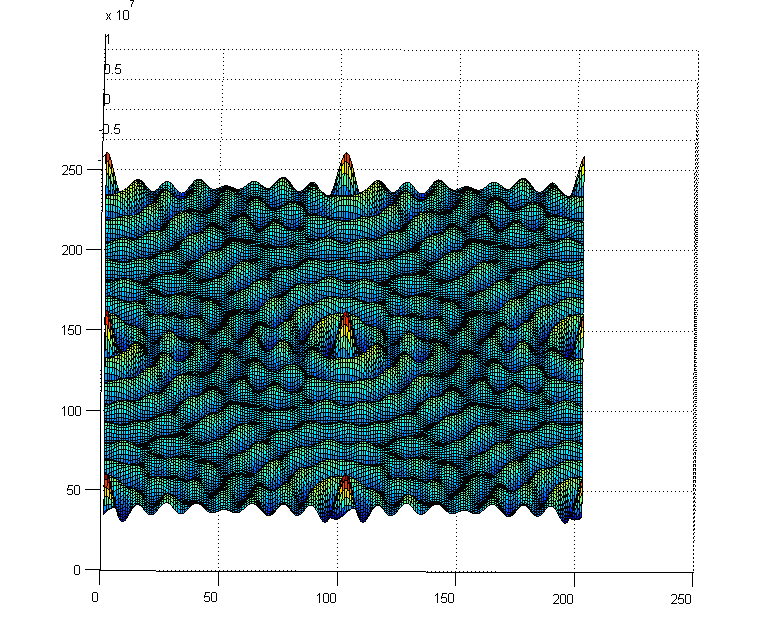
\includegraphics[width=1.00\textwidth]{autocorr50by50wav1000.png}
	\caption{Autocorrelation matrix for a sample $\Psi$.}
	\label{fig:autocorr50by50wav1000}
\end{figure}

\pagebreak

\subsection{Complex}

We then preform the same "randomness tests" as before obtaining the expected exponential distribution for $|\Psi|^{2}$,

\subsubsection{Gaussian point wise correlation}

We note that because the individual components of the waves were generated in the exact same way as with the real case (just separately) that individually they will follow a gaussian distribution.

\begin{figure}[hpt]
	\centering
		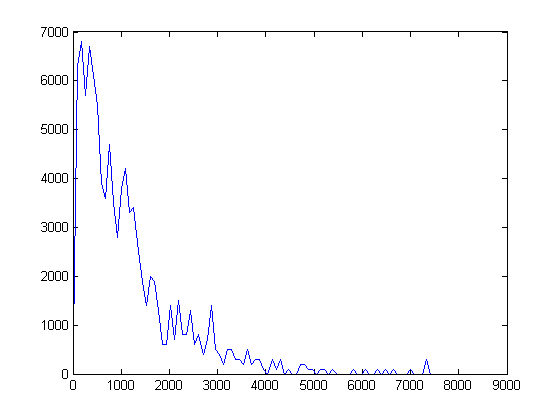
\includegraphics[width=1.00\textwidth]{randomdist1000p50by50wav1000C.png}
	\caption{Distribution of 1000 values of random points of a sample $|\Psi|^{2}$.}
	\label{fig:randomdist1000p50by50wav1000C}
\end{figure}

\pagebreak

\subsubsection{Autocorrelation matrix}

and the expected $J_{0}$ bessel like function for the autocorrelation matrix,

\begin{figure}[hpt]
	\centering
		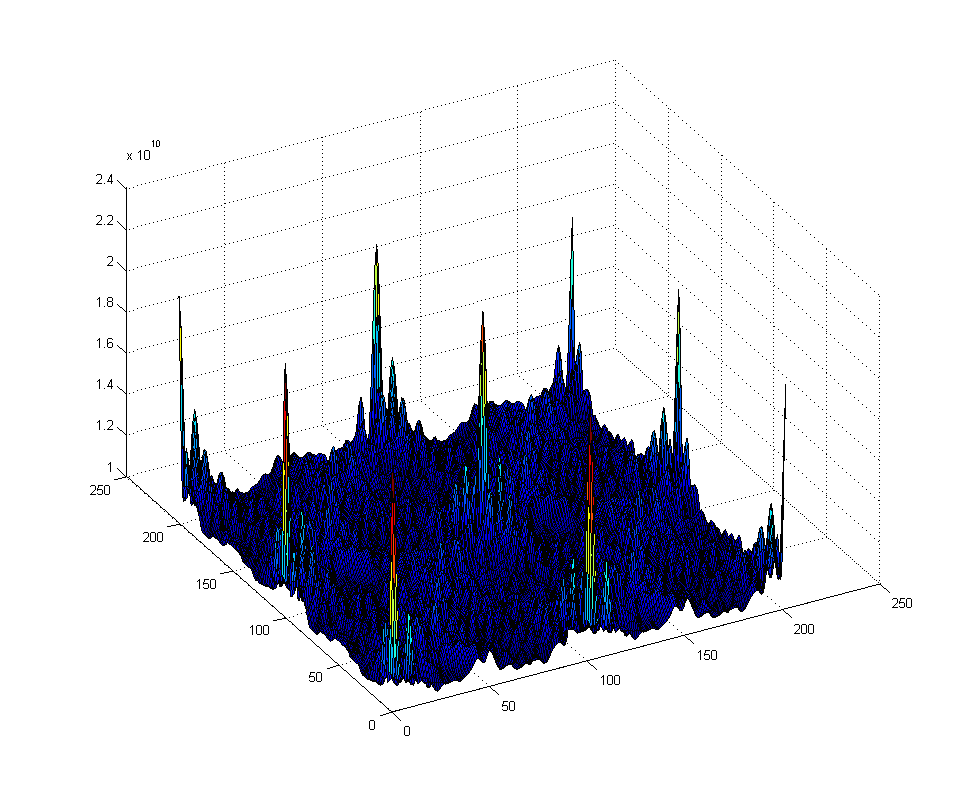
\includegraphics[width=1.00\textwidth]{autocorr50by50wav1000C.png}
	\caption{Autocorrelation matrix for a sample $|\Psi|^{2}$.}
	\label{fig:autocorr50by50wav1000C}
\end{figure}

\pagebreak

\begin{thebibliography}{99}
\bibitem{LH21} M.S. Longuet-Higgins, Phil. Trans. R. Soc. A \textbf{250}, 157 (1957)
\bibitem{AW75} A. Weinrib, B.I. Halperin, Phys. Rev. B \textbf{26}, 1362 (1982)
\bibitem{RA98} R. Aurich, A B\"acker, R. Schubert, M. Taglieber, Physica D \textbf{129}, 1 (1998)
\end{thebibliography}

\end{document}